\subsubsection{Terminology}
\label{sub:dl_terminology}

% AI, ML & DL confusion
In order to understand the concepts behind deep learning, the term has to be
separated from already mentioned areas machine learning and artificial
intelligence, as well as also common term \textit{neural networks}. 
These terms are often used interchangeably, but each defines a distinct area of 
research and they essentially mean different things.
\textbf{Artificial intelligence (AI)} is a research area that aims to understand
and build intelligent entities (often called \textit{agents}). Hence, AI touches the 
areas of philosophy, mathematics, psychology and computer science. Here, 
intelligence is defined as \textit{rational action}, which means that an agent aims
to perform the best possible action in a given setting~\footcite{Russell1995}.

In order to perform actions in an intelligent mannner, agents need to be able
to recognize patterns in observed data. The found patterns can then be used
by the agent to build up knowledge. This process is known as \textbf{machine
learning (ML)}~\footcite{Goodfellow2016}. In order to understand the methodology in
later chapters of this thesis, a more detailed examination of machine learning
problems is needed. Mitchell~\footcite[2]{Mitchell1997} offers the following 
definition for machine learning algorithms:

\begin{quote}
  A computer program is said to learn from experience E with respect to some
  class of tasks T and performance measure P, if its performance at tasks in T,
  as measured by P, improves with experience E.
\end{quote}

Following this definition, a machine learning algorithm can be classified along
three dimensions. Below, these dimensions are explained using the running
example of an algorithm that aims to predict house prices from advertisement data.
Such data might include the number of bedrooms, square footage and whether
the house includes a garage. Figure~\ref{fig:ml_classification} serves as an orientation and summary for
following remarks.

\begin{figure}[h]
  \centering
  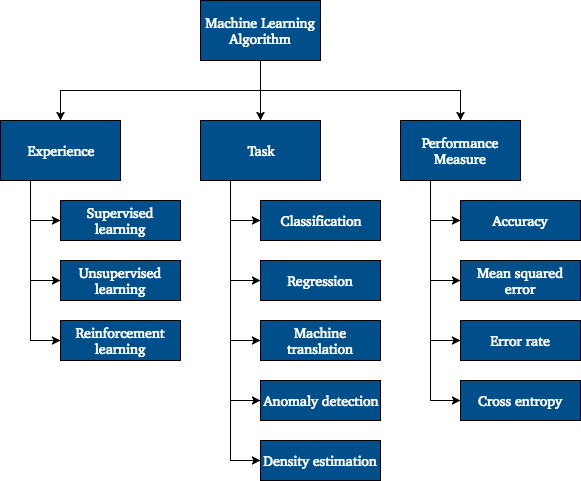
\includegraphics[height=10cm]{img/ml_classification}
  \caption{Classification dimensions of machine learning algorithms}
\label{fig:ml_classification}
\end{figure}

\paragraph{Task}

Machine learning is often used in settings where programs with fixed rules are
insufficient. Hence, the application of machine learning adds a more dynamic
component in order to perform a given task. Here, the task is usually to process
an \textit{example} which consists of a set of \textit{features}. Features are
attributes of an object that can be measured quantitatively~\footcite{Goodfellow2016}. 
In the example described above, the number of bedrooms is one the features of 
the house object. The task \textit{T} would then be to predict a price for this 
house. Depending on the type of the specific output variable this problem can 
be assigned to one of many groups of tasks (see Fig.~\ref{fig:ml_classification}). If the output was an
exact price (e.g. 1,000,000\$), this would constitute a \textbf{regression} task. 
Assuming the goal is to assign the house to a price interval (e.g., (500,000\$, 1,000,000\$]),
one would describe this as a \textbf{classification} problem. Other common tasks
can be derived from Figure 2.1. One such example would be \textbf{anomaly detection}, e.g.,
if the goal were to detect expensive houses in a neighborhood where house prices
are typically low. The task could also be to translate house descriptions from
English into other languages (\textbf{machine translation}) or to derive an
estimation of the underlying probability distribution of the data (\textbf{density estimation}).

\paragraph{Performance measure}

In order to perform a task \textit{T} better over time, the algorithm needs
a quantitative measure for its current performance. In the setting of
house price prediction, the algorithm should get feedback on the quality of its
predictions. For a regression problem a suitable performance measure would be 
the \textbf{mean squared error} over all training examples. Possible measures
for classification tasks would be \textbf{accuracy} (i.e., how many examples
were classified correctly?) or the \textbf{error rate} (i.e., how many
examples were classified incorrectly?). If the algorithm outputs class 
probabilities, \textbf{cross entropy} can be used to evaluate model
performance. Defining the correct performance measure can be more difficult
for more complex learning problems such as machine translation. The design of 
\textit{P} can influence the training process, e.g., if not all errors have the
same misclassification cost. Furthermore, machine learning models should be evaluated on unseen
data, i.e., data points that were not used for training the model. This way,
one derives a better estimate of the generalization abilities of the model~\footcite{Bishop2006, Goodfellow2016, Mitchell1997}.

\paragraph{Experience}

Machine learning algorithms can further be classified by the `kind of experience
they are allowed to have during the training process'~\footcite[104]{Goodfellow2016}.
In \textbf{unsupervised learning} settings the label for an example (also called
\textit{data point}) is unknown. For the house price prediction example this
would mean that real prices for the houses in the data set are not
available for training. Performing classification or regression tasks would
therefore not be feasible as the performance measure \textit{P} can not be
determined. Potential tasks in such an unsupervised learning setting would be
clustering (e.g., identifying similar houses), or performing density estimation
(e.g., to derive the probability for a given house price). In a broad sense these
kinds of algorithms aim to identify underlying distributions of data. Contrary, in 
\textbf{supervised learning} settings each example is associated with an 
observed output (usually called \textit{label} or \textit{target}). Hence, a
performance measure can be calculated for each data point, by which the
algorithm is able to improve its predictions over time (see above classification
and regression examples)~\footcite{Goodfellow2016, Bishop2006}. The third kind of
experience for a machine learning algorithm is a \textbf{reinforcement learning}
setting. Here, the algorithm does not rely on a fixed data set, but instead 
interacts with its environment steadily. It then learns from the feedback it
derives from these interactions. A common usecase for reinforcement
learning is the interaction of agents with the real environments, e.g.,
self-driving cars. In most of these settings collecting all data points is
insufficient or simply not feasible~\footcite{Sutton1998}.

It becomes obvious that the three dimesions are related, i.e., choices for a
specific dimension are conditioned on the other dimensions. Prior identification 
of all three dimensions is key in order to identify 
`well-defined learning problems'~\footcite[2--3]{Mitchell1997}. All developed 
learning algorithms in later chapters will also use this classification 
framework. 
